%**************************************************************************************
% License:
% CC BY-NC-SA 4.0 (http://creativecommons.org/licenses/by-nc-sa/4.0/)
%**************************************************************************************

\documentclass[notes]{beamer}

\mode<presentation> {

\usetheme{Madrid}

% Burnt orange
\definecolor{burntorange}{rgb}{0.8, 0.33, 0.0}
\colorlet{beamer@blendedblue}{burntorange}
% Pale yellow
\definecolor{paleyellow}{rgb}{1.0, 1.0, 0.953}
\setbeamercolor{background canvas}{bg=paleyellow}
% Secondary and tertiary palett
\setbeamercolor*{palette secondary}{use=structure,fg=white,bg=burntorange!80!black}
\setbeamercolor*{palette tertiary}{use=structure,fg=white,bg=burntorange!60!black}

% To remove the footer line in all slides uncomment this line
%\setbeamertemplate{footline}
% To replace the footer line in all slides with a simple slide count uncomment this line
%\setbeamertemplate{footline}[page number]

% To remove the navigation symbols from the bottom of all slides uncomment this line
%\setbeamertemplate{navigation symbols}{}
}

\usepackage{amsmath}
\usepackage{bm}
\usepackage{breqn}
\usepackage{cancel}
\usepackage{graphicx} % for figures
\usepackage{subcaption} % for subplots 
\usepackage[labelsep=space,tableposition=top]{caption}
\renewcommand{\figurename}{Fig.} 
\usepackage{cleveref}
\usepackage{caption,subcaption}% http://ctan.org/pkg/{caption,subcaption}
\usepackage{booktabs} % Allows the use of \toprule, \midrule and \bottomrule in tables
\usepackage{multirow}
\usepackage{tabularx}
\usepackage{siunitx}
\usepackage{cleveref}
\usepackage{xcolor}
\usepackage{empheq}
\usepackage[most]{tcolorbox}

\newtcbox{\mymath}[1][]{%
	nobeforeafter, math upper, tcbox raise base,
	enhanced, colframe=blue!30!black,
	colback=blue!30, boxrule=1pt,
	#1}

% To print 2 slides on a page
%\usepackage{handoutWithNotes}
%\pgfpagesuselayout{2 on 1}[border shrink=2mm]
%----------------------------------------------------------------------------------------
%	TITLE PAGE
%----------------------------------------------------------------------------------------
% The short title appears at the bottom of every slide, the full title is only on the title page
\title[CE394M: Cam-Clay]{CE394M: Critical State and Cam-Clay} 
\author{Krishna Kumar} % name
\institute[UT Austin] % institution 
{
University of Texas at Austin \\
\medskip
\textit{
  \url{krishnak@utexas.edu}} % Your email address
}
\date{\today} % Date, can be changed to a custom date

\begin{document}

\begin{frame}
\titlepage % title page as the first slide
\end{frame}

\begin{frame}
 % Table of contents slide, comment this block out to remove it
 \frametitle{Overview}
  %Throughout your presentation, if you choose to use \section{} and \subsection{} 
  %commands, these %will automatically be printed on this slide as an overview 
 \tableofcontents
\end{frame}

%----------------------------------------------------------------------------------------
% slides
%----------------------------------------------------------------------------------------
\section{Critical State Soil Mechanics}
%----------------------------------------------------------------------------------------
\begin{frame}
\frametitle{Critical State Soil Mechanics}
Roscoe et al., (1958), Schofield \& Worth (1968), Wood (1990):
\mode<beamer>{
	\begin{itemize}
		\item Provides a conceptual framework in which to interpret stress-strain-strength-volumetric strain response of soil.
		\item Started as a qualitative, rather than a mathematical model
		\item A unified framework of known or observed soil responses: drained / undrained / etc
	\end{itemize}
}
\mode<handout>{
	\vspace{6cm}
}
\end{frame}

%----------------------------------------------------------------------------------------
\begin{frame}
\frametitle{Critical state variables}
\noindent
\fboxsep=0pt
\noindent
\begin{minipage}[t]{0.65\linewidth}
	\begin{itemize}
		\item Mean stress: $p^\prime = \frac{\sigma_a^\prime  + 2 \sigma_r^\prime}{3} = p - u$.
		\item Deviatoric stress: $q = \sigma_a^\prime - \sigma_r^\prime = \sigma_a - \sigma_r$
		\mode<beamer>{
			\item Specific volume: $v = \frac{V_T}{V_s} = \frac{V_s + V_v}{V_s} = 1 + e$.
		}
		\mode<handout>{
			\vspace{1cm}
		}	
		
	\end{itemize}
\end{minipage}%
\hfill
\begin{minipage}[t]{0.35\linewidth}
	\begin{figure}
	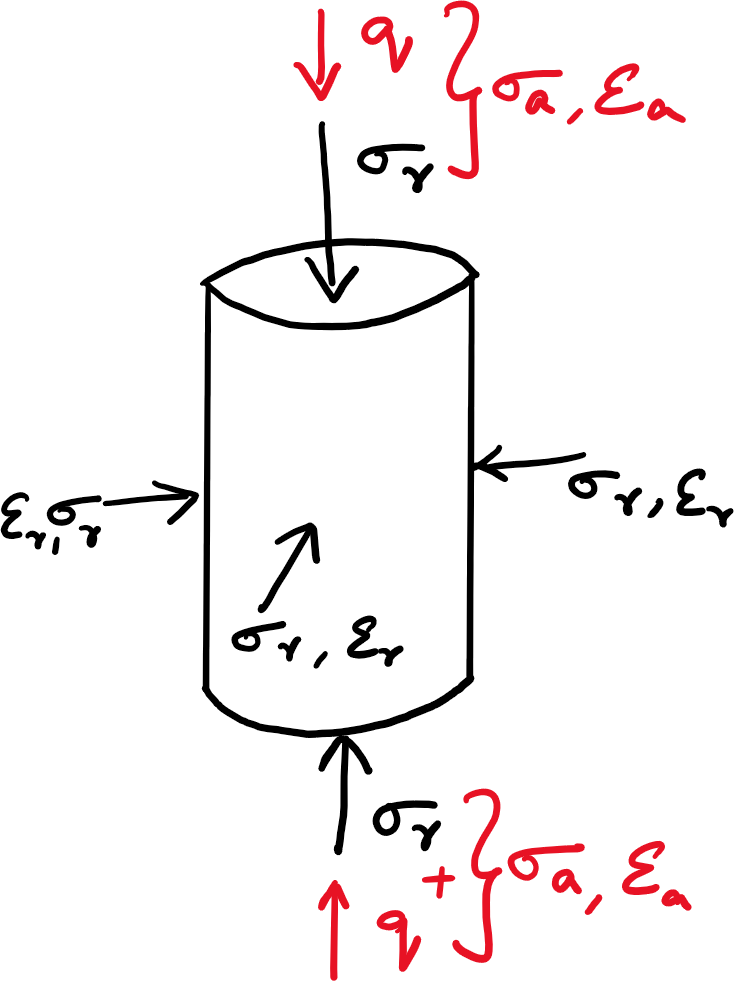
\includegraphics[width=0.9\textwidth]{figs/triaxial.png}
	\end{figure}
\end{minipage}	
\end{frame}

%----------------------------------------------------------------------------------------
\begin{frame}
\frametitle{Critical State Hypothesis: I}
Roscoe, Schofield \& Worth (1958): \textbf{At shear-failure, soil exists at a unique state}
\mode<beamer>{
	\begin{itemize}
		\item $d\varepsilon_s >> 0$ unlimited shear strain potential.
		\item $dp^\prime = dq = d\varepsilon_v = 0$ no change in $p^\prime, q, \varepsilon_v$.
		\item Critical state stress ratio: $\eta = q / p^\prime = const = M$ at failure $q = M p^\prime$.
	\end{itemize}
}
\mode<handout>{
	\vspace{3cm}
}
\begin{figure}
	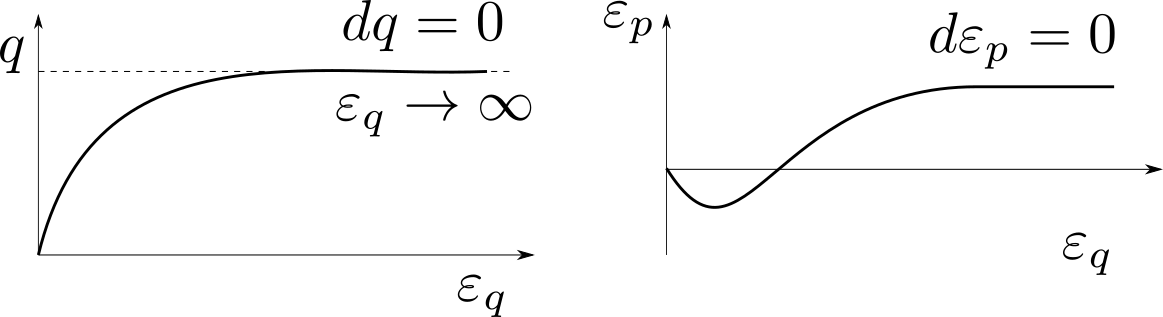
\includegraphics[width=0.9\textwidth]{figs/critical-state.png}
\end{figure}
\end{frame}
\note{Soil is sheared to a point where stresses are stationary $(dq = dp^\prime = 0)$ with no futher change in volume $(d\varepsilon_v = 0)$, unlimited shear strains $(d\varepsilon_s >> 0)$ and $q/p^\prime$ has a fixed value: \textbf{critical state}.

$M$ can be related to $phi^\prime$: $M = \frac{6\sin\phi^\prime}{3 - \sin\phi^\prime}$.
}


%----------------------------------------------------------------------------------------
\begin{frame}
\frametitle{Critical State Hypothesis: II}
\textbf{Critical state is a function of $q, p^\prime, v$. }
\begin{figure}
	\includegraphics[width=0.4\textwidth]{figs/critical-state-3d.png}
	\caption*{The CSL ($p^\prime, v, q$) space is given by the intersection of two planes: $q = Mp^\prime$ and a cruved vertical plane $v = \Gamma - \lambda \ln p^\prime$}
\end{figure}
\end{frame}

\note{Critical state curve connecting critical state points:
\begin{itemize}
	\item Crticial state line
	\item Defined in 3D but we'll look at projections into $q - p^\prime$ and $v - p^\prime$ space
\end{itemize}
}


%----------------------------------------------------------------------------------------
\begin{frame}
\frametitle{Critical State Hypothesis: II}
\textbf{Critical state is a function of $q, p^\prime, v$. }
\begin{figure}
	\includegraphics[width=\textwidth]{figs/critical-state-2d.png}
	\caption*{The CSL in (a) ($p^\prime, q$) plot and (b) ($p^\prime, v$) plot (isotropic normal compression line is shown in dashed)}
\end{figure}
\end{frame}

%----------------------------------------------------------------------------------------
\begin{frame}
\frametitle{Critical State Hypothesis: II}
\textbf{Critical state is a function of $q, p^\prime, v$. }
\begin{figure}
	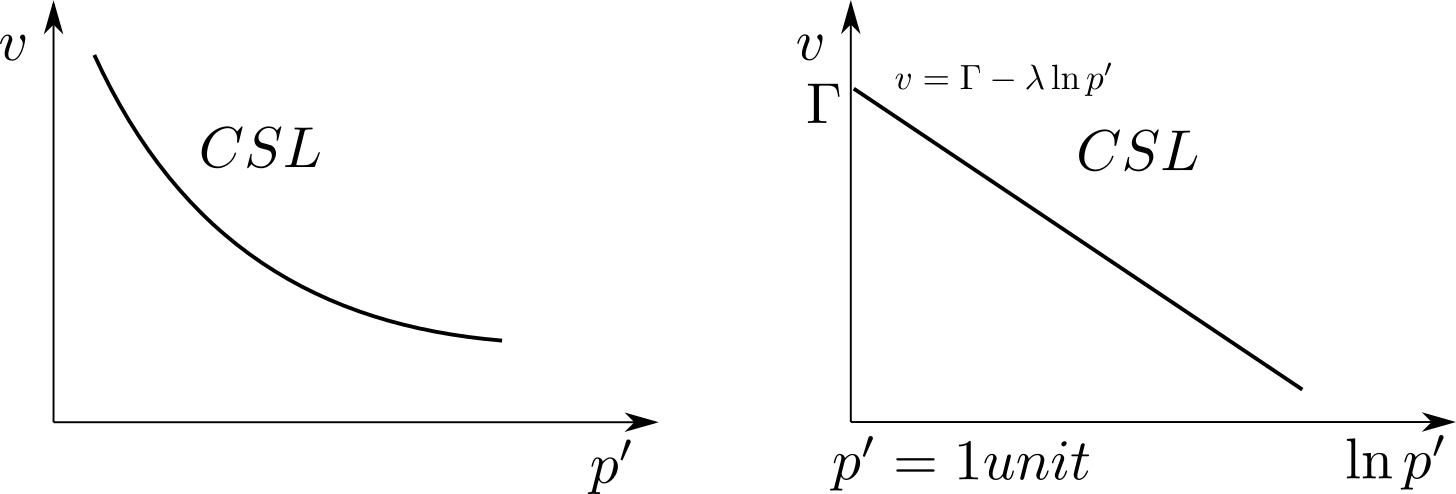
\includegraphics[width=\textwidth]{figs/v-lnp.png}
\end{figure}
\end{frame}

%----------------------------------------------------------------------------------------
\begin{frame}
\frametitle{Critical State Hypothesis: II}
\textbf{Critical state is a function of $q, p^\prime, v$. }
\begin{figure}
	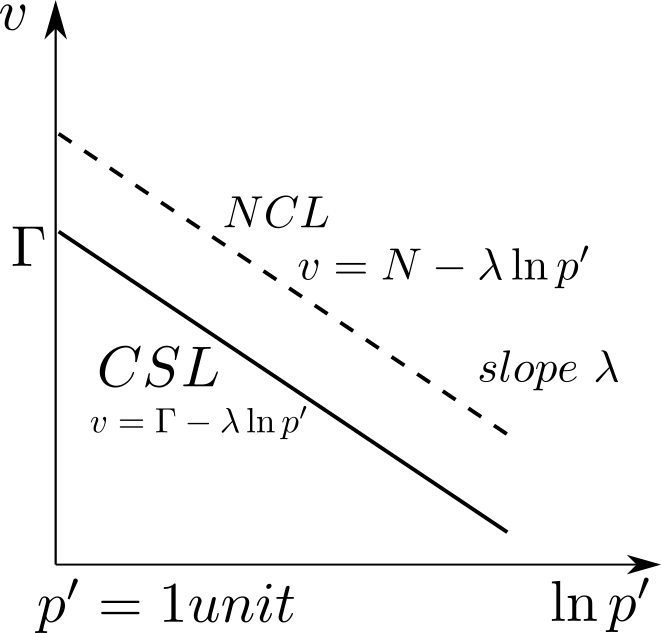
\includegraphics[width=0.6\textwidth]{figs/csl-ncl.png}
\end{figure}
\end{frame}

\note{
	Isotropic virgin compression line (VCL) $\eta = 0$. NCL is parallel to CSL. VCL is $\eta = 0$, while CSL $\eta = M$. Oedometer falls between VCL and CSL at a constant $\eta$: $0 < \eta < M$.
}


%----------------------------------------------------------------------------------------
\begin{frame}
\frametitle{Critical State Hypothesis: II}
\textbf{Critical state is a function of $q, p^\prime, v$. }
\begin{figure}
	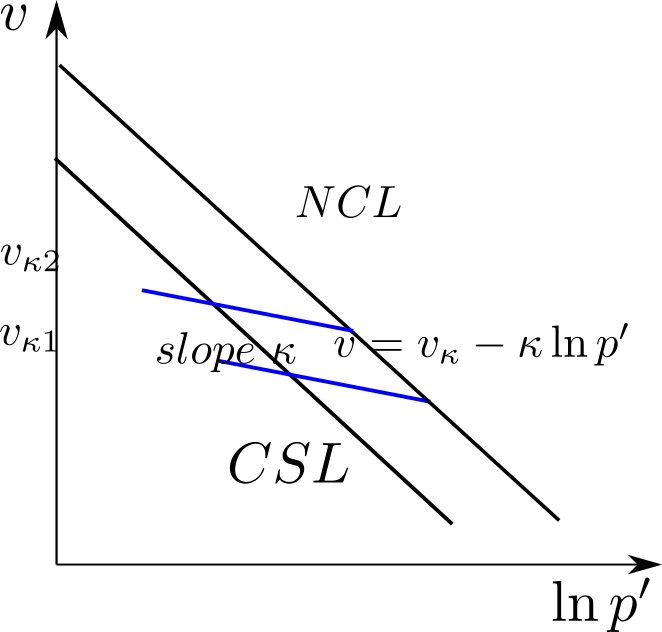
\includegraphics[width=0.65\textwidth]{figs/kappa.png}
\end{figure}
\end{frame}

\note{$v_\kappa$ depends on which $\kappa$ line you are on. $\kappa \ne c_r$ and $\lambda \ne C_c$}


%----------------------------------------------------------------------------------------
\begin{frame}
\frametitle{Stress paths $\sigma_3^\prime / \sigma_1^\prime = K_c = const$}
\begin{figure}
	\includegraphics[width=0.54\textwidth]{figs/stress-paths-kc.png}
\end{figure}
\end{frame}

%----------------------------------------------------------------------------------------
\begin{frame}
\frametitle{Clay behavior}
\begin{figure}
	\includegraphics[width=0.7\textwidth]{figs/clay-behavior.png}
\end{figure}
\end{frame}

%----------------------------------------------------------------------------------------
\begin{frame}
\frametitle{Critical state boundary surface}
\begin{figure}
	\includegraphics[width=0.45\textwidth]{figs/yieldsurface-3d.png}
\end{figure}
\end{frame}

%----------------------------------------------------------------------------------------
\begin{frame}
\frametitle{Summary of critical state behavior}
\mode<beamer>{
	\begin{itemize}
		\item Can only traverse NCL in one direction
		\item Can traverse RCL ($\kappa$-line) in both directions
		\item To move from one $\kappa$-line to another must move along NCL. Hence, plastic volumetric strains must occur.
		\item Critical state line is \textbf{NOT} a yield surface. It's where it's going but a lot of plastic straining is needed to get there. (if $CSL = F = 0$) then with associative flow rule $d\varepsilon_v^p \ne0$ at critical state. Real $F$ is horizontal at critical state.
	\end{itemize}
}
\mode<handout>{
	\vspace{6cm}
}
\end{frame}


%----------------------------------------------------------------------------------------
\section{Cam-Clay}

%----------------------------------------------------------------------------------------

%----------------------------------------------------------------------------------------
\begin{frame}
\frametitle{Stress - dilatancy theory (Taylor, 1948)}
\begin{figure}
	\includegraphics[width=0.45\textwidth]{figs/direct-shear.png}
\end{figure}
\mode<beamer>{
	Work in friction and dilation:
	\begin{equation*}
		\tau dx - \sigma_n^\prime dy = \mu \sigma_n^\prime dx
	\end{equation*}
}
\mode<handout>{
	\vspace{3cm}
}
\end{frame}

\note{Taylor (1948) proposed
	a stress-dilatancy theory based on the work balance equation: The external work
	corresponds to the product of the measured displacements and forces (assuming that the elastic
	deformation is negligible). The internal work corresponds to the frictional force.}


%----------------------------------------------------------------------------------------
\begin{frame}
\frametitle{Formulation of elasto-plastic Cam-Clay (OCC): Yield function}
Derived from work consideration:
\begin{figure}
	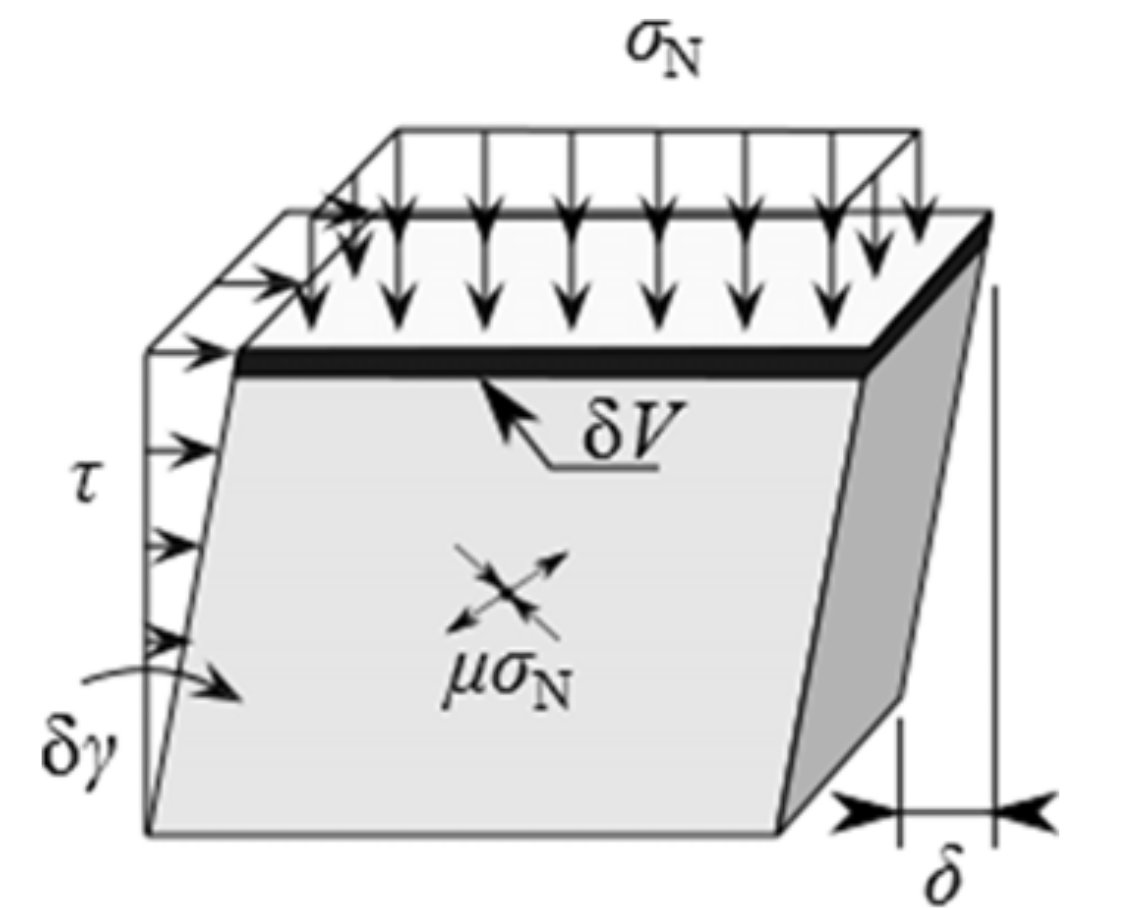
\includegraphics[width=0.4\textwidth]{figs/simple-shear.png}
\end{figure}

\mode<beamer>{
	External work: $\delta w_{ext}^p = p^\prime d\varepsilon_v^p + q d \varepsilon_s^p$
	Assume that the internal work is dissipated by internal friction only: $\delta w_{int}^p = M p^\prime d \varepsilon_s^p$

	\begin{equation*}
		\delta w_{ext}^p = p^\prime d\varepsilon_v^p + q d \varepsilon_s^p = M p^\prime d \varepsilon_s^p = \delta w_{int}^p
	\end{equation*}
}
\mode<handout>{
	\vspace{3cm}
}
\end{frame}
\note{This dissipation function can be regarded simply as generalisation of Taylor's equation. It should be  noted that both Taylor's equation and Cam-Clay dissipation function equation assume that when   there is some combination of volumechange ($dy$ or $\partial \varepsilon_v$) and of shear distortion ($dx$ or $\partial \varepsilon_s$) it is the shear strain that determines the dissipation rate. The dilation or volume change is a geometrical consequence of interlocking, and does not appear explicitly in the dissipation function. }


%----------------------------------------------------------------------------------------
\begin{frame}
\frametitle{Cam-Clay (OCC): Stress dilatancy relation}
\begin{equation*}
p^\prime d\varepsilon_v^p + q d \varepsilon_s^p = M p^\prime d \varepsilon_s^p
\end{equation*}
Rearranging the terms (divide by $p^\prime d\varepsilon_s^p$):
\mode<beamer>{
	\begin{equation*}
	\frac{d\varepsilon_v^p }{d\varepsilon_s^p } = M - \frac{q}{p^\prime} = M - \eta
	\end{equation*}
	Where $\eta = q/p^\prime$ is defined as the stress-ratio. This equation is known as the dilatancy expression and expresses the ratio in plastic volumetric and deviatoric components. 
	
	
	\begin{align*}
	q/p<M: \quad & \frac{d\varepsilon^p\varepsilon_v}{d\varepsilon^p_q} > 0 \rightarrow \quad d\varepsilon^p\varepsilon_v > 0 \quad \text{Contractive response}\\
	q/p > M: \quad &	\frac{d\varepsilon^p\varepsilon_v}{d\varepsilon^p_q} > 0 \rightarrow \quad d\varepsilon^p\varepsilon_v < 0 \quad\text{Dilative response} \\
	q/p = M: \quad & d\varepsilon^p\varepsilon_v  = 0 \quad \text{No volume change}
	\end{align*}
}
\mode<handout>{
	\vspace{6cm}
}
\end{frame}

\note{The critical state is defined by an absence of volume change or, in other words, a nil dilatancy
conditions. Therefore, at critical state, the stress-dilatancy rule yields to the critical state condition $\eta = M$.}


%----------------------------------------------------------------------------------------
\begin{frame}
\frametitle{Cam-Clay (OCC): flow-rule}
The original idea was very simple. The yield locus must be such that each associated flow rule $(\delta \varepsilon_v, \delta \varepsilon_s)$ would be orthogonal to the tangent to the yield locus.

\noindent
\fboxsep=0pt
\noindent
\begin{minipage}[t]{0.65\linewidth}
	\mode<beamer>{
	\begin{equation*}
		\frac{\delta \varepsilon_v}{\delta \varepsilon_s} = - \frac{\delta \varepsilon_s}{\delta \varepsilon_v^\prime}
	\end{equation*}
	From stress dilation condition:
	\begin{equation*}
		\frac{dq}{dp^\prime} = - (M - \eta) = -M + \eta
	\end{equation*}
	Integrating we obtain:
	\begin{equation*}
		q = M p^\prime \ln\left(\frac{p_c^\prime}{p^\prime}\right)
	\end{equation*}
	Where $p^\prime_c$ is the value of $p^\prime$ at $q = 0$.
	}
	\mode<handout>{
		\vspace{4cm}
	}
	
\end{minipage}%
\hfill
\begin{minipage}[t]{0.35\linewidth}
	\begin{figure}
		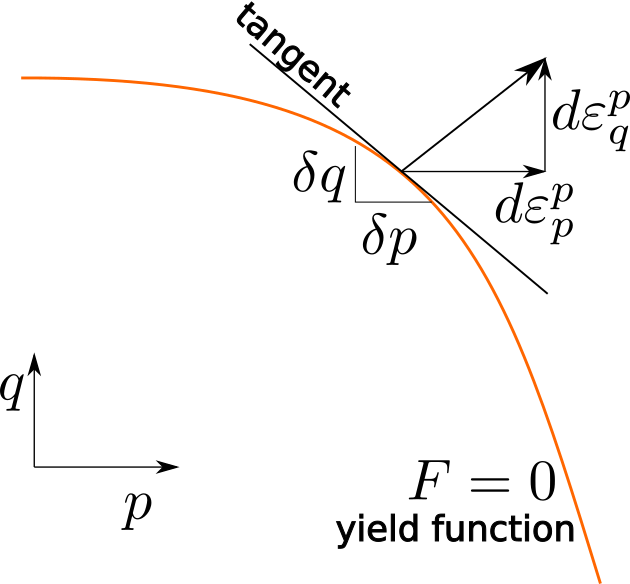
\includegraphics[width=\textwidth]{figs/flow-rule.png}
	\end{figure}
\end{minipage}
\end{frame}

\note{\textbf{Original Cam-Clay integration}
	\begin{equation*}
	\eta = q/p \quad \rightarrow d\eta = \frac{\partial \eta}{\partial q} dq + \frac{\partial \eta}{\partial p^\prime} dp^\prime
	\end{equation*}

Which gives:
	\begin{equation*}
		d\eta = \frac{dq}{p} - \frac{q}{p^2} dp \rightarrow \quad dq = p d\eta + \eta dp
	\end{equation*}

We know from flow rule and orthogonality: $dq = dp (-M + \eta)$

Equating the above 2 equations:
	\begin{align*}
		dp = & p d\eta + \eta dp =  dp (-M + \eta) \\
		& p d \eta = -M dp \rightarrow \quad deta = -M \frac{dp}{p}
	\end{align*}
Integrating this expression we obtain:
	\begin{equation}
		\eta = -M \ln p + C
	\end{equation}
}


\note{\textbf{Original Cam-Clay integration}
	\begin{equation}
	\eta = -M \ln p + C
	\end{equation}
To find the constants, for $\eta = 0$, we get $p = p_c$:
	\begin{equation*}
		0 = -M \ln p_c + C \quad C = M \ln p_c
	\end{equation*}
Which gives:
	\begin{align*}
		\eta &= M \ln p_c - M \ln p \\
		q/p &= M \ln \left(p_c/p\right)
	\end{align*}
Yield function:
	\begin{equation*}
		F = q - M p^\prime \ln(p_c^\prime / p^\prime) = 0
	\end{equation*}
}

%----------------------------------------------------------------------------------------
\begin{frame}
\frametitle{Cam-Clay (OCC): Elastic properties}
\noindent
\fboxsep=0pt
\noindent
\begin{minipage}[t]{0.65\linewidth}
	\mode<beamer>{
		Swelling: $\delta v_\kappa = \kappa \ln (p^\prime_1 /p^\prime_2)$
		
		Elastic bulk modulus: $K = \frac{dp^\prime}{d\varepsilon_v}$.
		
		We know the volumetric compression on elastic reloading line:
		
		$dv = -\kappa \frac{dp^\prime }{p^\prime}$
		
		\begin{equation*}
		d \varepsilon_v = \frac{-de}{1 + e_0} = \frac{-dv}{v_0} = \frac{\kappa}{v_0}\frac{dp^\prime}{p^\prime}
		\end{equation*}
		
		$K^\prime$ is not constant: $K^\prime = K^\prime (p^\prime)$. Assuming a constant poisson ratio: $\nu$, so $G, K$ vary.
		
		\begin{equation*}
			K = \frac{dp}{d\varepsilon_v} = \frac{v_o p^\prime}{\kappa} = \frac{(1+e_0)p^\prime}{\kappa}
		\end{equation*}	
	}
	\mode<handout>{
		\vspace{6cm}
	}
	
\end{minipage}%
\hfill
\begin{minipage}[t]{0.35\linewidth}
	\begin{figure}
		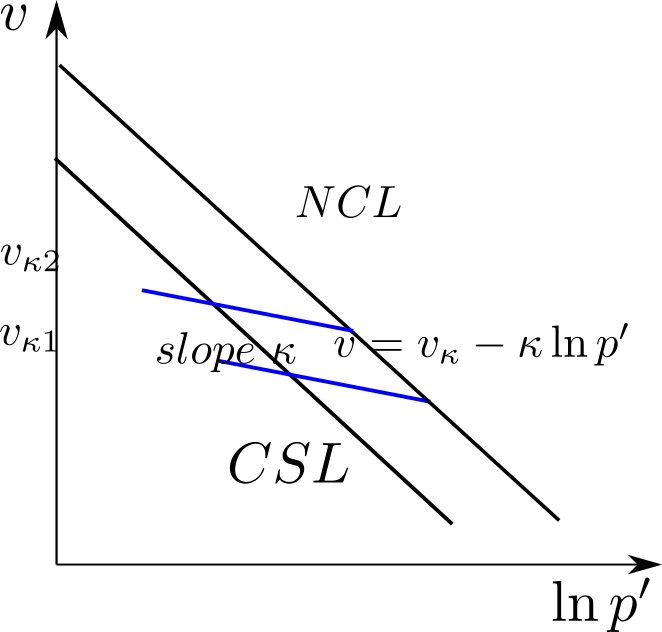
\includegraphics[width=\textwidth]{figs/kappa.png}
	\end{figure}
\end{minipage}
\end{frame}

\note{
	\textit{Observation}: 
	\begin{itemize}
		\item Stiffness $K$ increases with $p^\prime$: correct.
		\item Stiffness increases with void ratio (not right)!
	\end{itemize}
	
	\textit{Note: }The original derivation assumed that there were no recoverable (elastic) shear strains so $G = \infty$. We can find the stress-strain relationships for a single element in this case, but for a finite element forumulation we need to have a finite $G^e$. So there are two options:
	\begin{itemize}
		\item Define $G = f(e, p^\prime)$.
		\item Use a constant ``elastic'' Poisson ratio. Ratio between the shear and bulk modulus is constant. $2G/K = const$.
	\end{itemize}
	The first alternative has the shortcoming that depending on the choice of $G$ we may have unreasonable values of the ``elastic'' Poisson's ratio. I prefer the second choice.
}



%----------------------------------------------------------------------------------------
\begin{frame}
\frametitle{Cam-Clay (OCC): Hardening law}
We need to define how the yield surface hardens as plastic work is being performed. Only ``\textit{memory}'' parameter in our yield surface is the size: $p_c^\prime$.

From the isotropic NCL:
	\begin{equation*}
	d\varepsilon_v = \frac{-dv}{v} = \frac{-de}{1 + e} = \frac{+\lambda}{v} \frac{dp_c^\prime}{p_c^\prime}
	\end{equation*}

But the increment in elastic volumetric strain is:
	\begin{equation*}
	d\varepsilon_v^e = \left(\frac{-dv}{v}\right)^{elastic} = + \frac{\kappa}{v}\left(\frac{dp_c^\prime}{p_c^\prime}\right)
	\end{equation*}

\end{frame}


%----------------------------------------------------------------------------------------
\begin{frame}
\frametitle{Cam-Clay (OCC): Hardening law}
\noindent
\fboxsep=0pt
\noindent
\begin{minipage}[t]{0.65\linewidth}
\begin{align*}
d\varepsilon_{vol} & = - \frac{de}{(1 + e)} \\
   & = \frac{\kappa}{(1 + e)}\frac{dp^\prime}{p^\prime} + \frac{\lambda - \kappa}{(1 + e)}\frac{dp_c^\prime}{p_c^\prime} \\
   & = elastic + plastic\\
   & = d\varepsilon_{vol}^e + d\varepsilon_{vol}^p
\end{align*}
Therefore the increment of $p_c$ can be related to the increment of plastic volumetric strain:
\begin{align*}
d\varepsilon_v^p & = 	d\varepsilon_v - 	d\varepsilon_v^e = (\lambda - \kappa)\left(\frac{dp_c^\prime}{p_c^\prime}\right) \\
dp_c^\prime & = \left(\frac{v\cdot p_c^\prime}{(\lambda - \kappa)}\right) \cdot d \varepsilon_v^p
\end{align*}
\end{minipage}%
\hfill
\begin{minipage}[t]{0.35\linewidth}
	\begin{figure}
		\includegraphics[width=0.9\textwidth]{figs/hardening.png}
	\end{figure}
\end{minipage}
\end{frame}




%----------------------------------------------------------------------------------------
\begin{frame}
\frametitle{Cam-Clay (OCC): Hardening law}
We have seen that the hardening law:

\begin{equation*}
H = - \left(\frac{\partial F}{\partial Wp}\right)\left(\frac{\partial Wp}{\partial \varepsilon^p}\right)^T\cdot\frac{\partial G}{\partial \sigma}
\end{equation*}
$W_p$ is the vector of memory parameters. In our case, the CC model has only one parameter:\mode<beamer>{ $p_c^\prime$ and it's variation is only a function of the plastic volumetric strain. So:}
\mode<beamer>{
\begin{equation*}
H = - \left(\frac{\partial F}{\partial p_c^\prime}\right)\left(\frac{\partial p_c^\prime}{\partial \varepsilon^p}\right)^T\cdot\frac{\partial G}{\partial \sigma}
\end{equation*}	
}
\mode<handout>{
\vspace{1cm}
}
\end{frame}



%----------------------------------------------------------------------------------------
\begin{frame}
\frametitle{Cam-Clay (OCC): Hardening law}
We know:
\begin{align*}
\frac{\partial F}{\partial p_c^\prime} & = -M p^\prime / p_c^\prime \\
%
\frac{\partial p_c^\prime}{\partial \varepsilon^p} & = \frac{v}{(\lambda - \kappa)}p^\prime_c \\
%
\frac{\partial G}{\partial \sigma} & = P_p = Q_p = M - \eta
\end{align*}	

\begin{empheq}[box=\tcbhighmath]{equation*}	H = - \left(\frac{\partial F}{\partial p_c^\prime}\right)\left(\frac{\partial p_c^\prime}{\partial \varepsilon^p}\right)^T\cdot\frac{\partial G}{\partial \sigma} = M \frac{(M - \eta)}{(\lambda - \kappa)} \cdot (1 + e) \cdot p^\prime
\end{empheq}	
\end{frame}


%----------------------------------------------------------------------------------------
\begin{frame}
\frametitle{Deformations under an applied stress path}
\noindent
\fboxsep=0pt
\noindent
\begin{minipage}[t]{0.48\linewidth}
	\begin{figure}
	\includegraphics[width=\textwidth]{figs/elastic.png}
	\caption*{$P_{0B}^\prime > P_{0A}^\prime$ Elastic}
	\end{figure}	
\end{minipage}	%
\hfill
\begin{minipage}[t]{0.48\linewidth}
	\begin{figure}
		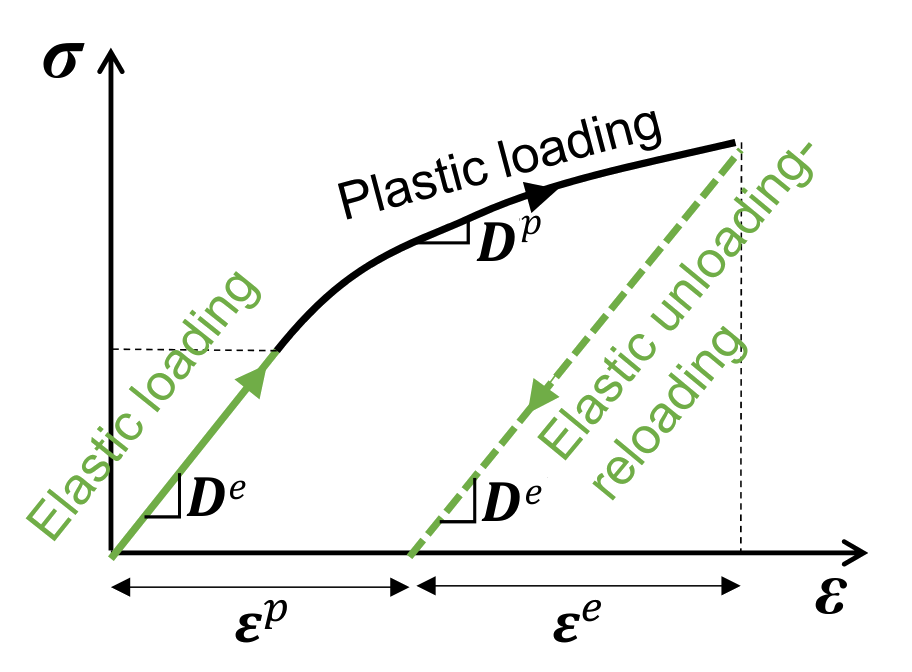
\includegraphics[width=\textwidth]{figs/elasto-plastic.png}
		\caption*{$P_{0B}^\prime < P_{0A}^\prime$ Elasto-plastic}
	\end{figure}
\end{minipage}	
\end{frame}


%----------------------------------------------------------------------------------------
\begin{frame}
\frametitle{Hardening law}
\noindent
\fboxsep=0pt
\noindent
\begin{minipage}[t]{0.49\linewidth}
	\begin{figure}
		\includegraphics[width=0.9\textwidth]{figs/occ-hardening.png}
	\end{figure}	
\end{minipage}	%
\hfill
\begin{minipage}[t]{0.49\linewidth}
	\mode<beamer>{
	\begin{itemize}
		\item \textcolor{purple}{$\eta < M \rightarrow d\varepsilon_p^p > 0 \quad dp^\prime > 0$ Yield surface ``\textit{expands}''}
		\item \textcolor{orange}{$\eta > M \rightarrow d\varepsilon_p^p < 0 \quad  dp^\prime < 0$ Yield surface ``\textit{contracts}''}
		\item \textcolor{green}{$\eta = M \rightarrow d\varepsilon_p^p = 0 \quad  dp^\prime =0$ Yield surface ``\textit{constant}''}
	\end{itemize}
	}
	\mode<handout>{
		\vspace{6cm}
	}
\end{minipage}	
\end{frame}

%----------------------------------------------------------------------------------------
\begin{frame}
\frametitle{Stress-strain relation in ($p^\prime, q$) and ($\varepsilon_v, \varepsilon_s$) drained TX}
\begin{enumerate}
	\item Give strain and/or stress increments
	\item Check if the current stress state is inside the yield surface or outside the yield surface $q/p^\prime = M \ln (p_c/p^\prime)$
	\begin{enumerate}
		\item If Elastic (stress inside yield surface):
		\begin{equation*}
		\begin{bmatrix}
		d\varepsilon_v \\
		d\varepsilon_s \\
		\end{bmatrix} = %
		%
		\begin{bmatrix}
		1/K & 0 \\
		0 & 1/3G\\
		\end{bmatrix} %
		\begin{bmatrix}
		dp^\prime \\
		dq\\
		\end{bmatrix}
		\end{equation*}
		\item If Elastic-plastic (stress on the yield surface)
		\begin{equation*}
		\begin{bmatrix}
		d\varepsilon_v \\
		d\varepsilon_s \\
		\end{bmatrix} = %
		%
		D^{ep}
		%
		\begin{bmatrix}
		dp^\prime \\
		dq\\
		\end{bmatrix}
		\end{equation*}		
		\begin{equation*}
		D^{ep} =\left[
		\begin{bmatrix}
		1/K & 0 \\
		0 & 1/3G\\
		\end{bmatrix} + %
		%
		\frac{1}{Mp^\prime}%
		\frac{(\lambda - \kappa)}{(1+e_0)}%
		%
		\begin{bmatrix}
		M - (q/p^\prime) & 1     \\
		1 & 1/(M - (q/p^\prime)) \\
		\end{bmatrix}
		\right]
		\end{equation*}
	\end{enumerate}
	\item Compute the unknown stress or strain increments and update the stress and strains
	\item If plastic deformation, update $p_c$ to satisfy Cam-Clay yield surface
	\item Go back to step 1
\end{enumerate}
\end{frame}


%----------------------------------------------------------------------------------------
\begin{frame}
\frametitle{Stress-strain relation in ($p^\prime, q$) and ($\varepsilon_v, \varepsilon_s$) undrained TX}
$d\varepsilon_v = d\varepsilon_a + 2 d\varepsilon_r = 0$ (constant volume)

$d\varepsilon_s = (2/3)(d\varepsilon_a - d\varepsilon_r) = (2/3)(d\varepsilon_a - (-0.5 d\varepsilon_a)) = d\varepsilon_a$
\begin{enumerate}
\item Give axial strain increment $d\varepsilon_a$ or $dq$
\item Check if the current stress state is inside the yield surface or outside the yield surface $q/p^\prime = M \ln (p_c/p^\prime)$
\begin{itemize}
	\item If Elastic (stress inside yield surface):
	\begin{equation*}
	\begin{bmatrix}
	d\varepsilon_v \\
	d\varepsilon_s \\
	\end{bmatrix} = %
	%
	\begin{bmatrix}
	1/K & 0 \\
	0 & 1/3G\\
	\end{bmatrix} %
	\begin{bmatrix}
	dp^\prime \\
	dq\\
	\end{bmatrix}
	\end{equation*}
	$d\varepsilon_v =$ from the first equation gives $dp^\prime = 0$. This means that the effective stress path is fixed to go in the vertical direction in $p^\prime - q$ space irrespective of any total stress path. 
	
	The second equation gives $d\varepsilon_s$ for a given $dq$ or $dq$ for a $d\varepsilon_s$.
\end{itemize}
\end{enumerate}
\end{frame}


%----------------------------------------------------------------------------------------
\begin{frame}
\frametitle{Stress-strain relation in ($p^\prime, q$) and ($\varepsilon_v, \varepsilon_s$) undrained TX}		
\begin{enumerate}
\setcounter{enumi}{3}
\item 

\begin{itemize}
\item If Elastic-plastic (stress on the yield surface)
\begin{equation*}
\begin{bmatrix}
d\varepsilon_v \\
d\varepsilon_s \\
\end{bmatrix} = %
%
D^{ep}
%
\begin{bmatrix}
dp^\prime \\
dq\\
\end{bmatrix}
\end{equation*}		
\begin{equation*}
D^{ep} =\left[
\begin{bmatrix}
1/K & 0 \\
0 & 1/3G\\
\end{bmatrix} + %
%
\frac{1}{Mp^\prime}%
\frac{(\lambda - \kappa)}{(1+e_0)}%
%
\begin{bmatrix}
M - (q/p^\prime) & 1     \\
1 & 1/(M - (q/p^\prime)) \\
\end{bmatrix}
\right]
\end{equation*}
$d\varepsilon_v = 0$ and $d\varepsilon_s = d\varepsilon_a$ give $dp^\prime$ and $dq$ 

or 

$d\varepsilon_v = 0$ and $dq$ gives $d\varepsilon_s(=d\varepsilon_a)$ and $dp^\prime$.
\end{itemize}
\item Update the stress and strain. The difference between the total mean pressure $p$ and the effective mean pressure will give the pore pressure.
\item If plastic deformation, update $p_c$ to satisfy Cam-Clay yield surface.
\item Go back to step 1
\end{enumerate}
\end{frame}


%----------------------------------------------------------------------------------------
\begin{frame}
\frametitle{Limitations of original Cam-Clay}
\mode<beamer>{
	\begin{enumerate}
		\item For an isotropically normally consolidated (saturated clay) specimen in TXC: Overpredicts the excess pore-pressure at failure.
		\item Yield surface / plastic potential function produces too much shearing at low stress-ratios. At low stress ratio you would expect mostly plastic volumetric strains rather than deviatoric stress.
		\item Yield surface is discontinous at the hydrostatic axis. 
		\item Overpredicts $K_0$ for a normally consolidated clay under 1D loading. For low $\phi_cs$ we get $K_0$ larger than 1 (unrealistic).
		\item Other modes of shearing?
		\item Anisotropy?
	\end{enumerate}
}
\mode<handout>{
	\vspace{6cm}
}
\end{frame}

\note{
	\begin{figure}
		\includegraphics[width=0.45\textwidth]{figs/camclay-limitations.png}
	\end{figure}
}



%----------------------------------------------------------------------------------------
\section{Modified Cam-Clay}
%----------------------------------------------------------------------------------------
\begin{frame}
\frametitle{What can we change?}
\mode<beamer>{
	\begin{enumerate}
		\item Yield function (yes)
		\item Elastic constants (not really) ~ controlled by the compression model.
		\item Flow rule (for associated models it is tied to the yield function).
		\item Hardening laws (~ constrained already by the compression model)
	\end{enumerate}
}
\mode<handout>{
	\vspace{6cm}
}
\end{frame}


%----------------------------------------------------------------------------------------
\begin{frame}
\frametitle{MCC: Yield function}
Derived from work considerations (Burland 1965, Roscoe and Burland 1968):
	\begin{equation*}
	dW_{int}^p = p \sqrt{(d\varepsilon_v^p)^2 + (M d\varepsilon_s^p)^2}
	\end{equation*}
This is the new equation describing the energy dissipated by the soil. Following similar arguments to CC:
\begin{equation*}
	dW_{ext}^p = p d \varepsilon_v^p + q d \varepsilon_s^p = p \sqrt{(d\varepsilon_v^p)^2 + (M d\varepsilon_s^p)^2} = dW_{int}^p
\end{equation*}
Squaring and re-arranging the terms:
\begin{equation*}
	\frac{d\varepsilon_v^p}{d\varepsilon_s^p} = \frac{M^2 - \eta^2}{2 \eta} = -\frac{dq}{dp^\prime}
\end{equation*}
Assuming an associative flow rule gives an elliptic yield surface:
\begin{empheq}[box=\tcbhighmath]{equation*}	
F(q, p) = q^2 - M^2 p^2 \left(\frac{p_c^\prime}{p^\prime} - 1\right) = 0
\end{empheq}	
\end{frame}

\note{
	\begin{equation*}
	\frac{d\varepsilon_v^p}{d\varepsilon_s^p} = \frac{M^2 - \eta^2}{2 \eta}
	\end{equation*}
	This is referred to as the dilatancy expression. In contrast to the original Cam-Clay, this equation predicts only plastic volumetric strain at $\eta = 0$ (isotropic state).
}

\note{
	\begin{figure}
		\includegraphics[width=0.45\textwidth]{figs/mcc-pc-pcs.png}
	\end{figure}
	For the MCC we can find the value of $p_{cs}$ the stress corresponding to the critical stress at CS: $q_{cs} = M p^\prime_{cs}$ and should be on the yield surface: $(M p^\prime_{cs})^2 = M^2 (p^\prime_{cs})^2 \left(\frac{p_c^\prime}{p_{cs}^\prime} -1 \right) \qquad \frac{p_c^\prime}{p_{cs}^\prime}  = 2 \rightarrow \quad p_{cs}^\prime =  p_c^\prime / 2$
}


%----------------------------------------------------------------------------------------
\begin{frame}
\frametitle{OCC v MCC}
	\begin{figure}
	\includegraphics[width=0.95\textwidth]{figs/occ-mcc.png}
\end{figure}
\end{frame}

%----------------------------------------------------------------------------------------
\begin{frame}
\frametitle{MCC: Stress-strain relationship}
\begin{figure}
	\includegraphics[width=0.8\textwidth]{figs/mcc-stress-strain.png}
\end{figure}
\end{frame}

%----------------------------------------------------------------------------------------
\begin{frame}
\frametitle{MCC: I}
\begin{figure}
	\includegraphics[width=0.8\textwidth]{figs/mcc-1.png}
\end{figure}
\end{frame}

%----------------------------------------------------------------------------------------
\begin{frame}
\frametitle{MCC: II}
\begin{figure}
	\includegraphics[width=0.8\textwidth]{figs/mcc-2.png}
\end{figure}
\end{frame}


%----------------------------------------------------------------------------------------
\section{Cam-Clay material properties determination}
%----------------------------------------------------------------------------------------
\begin{frame}
\frametitle{Cam-Clay material properties determination: I}
\textbf{Test required}
\begin{enumerate}
	\item Slow drained or undrained test with pore pressure measurement at different preconsolidation pressure. Test must be taken to very large strains to reach to the critical state.
	\item Isotropic consolidateion test or incrementental loading consolidation test.
\end{enumerate}


\noindent
\fboxsep=0pt
\noindent
\begin{minipage}[t]{0.65\linewidth}
\textbf{Slope of failure line: $M$}
\textbf{If $\phi_{cs}$ is assumed to be constant, then $M$ is not constant.
}
\begin{itemize}
	\item In TXC: $M_{TXC} = \frac{6 \sin \phi_{cs}}{3 - \sin \phi_{cs}}$
	\item In TXE: $M_{TXE} = \frac{6 \sin \phi_{cs}}{3 + \sin \phi_{cs}}$
	\item In PS: $M_{PS} = 2 \sin \phi_{cs}$ 
	
	(assuming $\sigma_2 \approxeq \frac{\sigma_1 + \sigma_3}{2})$
\end{itemize}

\end{minipage}%
\hfill
\begin{minipage}[t]{0.35\linewidth}
	\begin{figure}
		\includegraphics[width=0.9\textwidth]{figs/M-qp.png}
	\end{figure}
\end{minipage}	
\end{frame}

%----------------------------------------------------------------------------------------
\begin{frame}
\frametitle{Cam-Clay material properties determination: II}
\textbf{$\lambda$ and $\kappa$: Compression index and swelling index}
\begin{enumerate}
	\item Use isotropic consolidation. Plot in $v-\ln p^\prime$ plane. Measure $\lambda$ \& $\kappa$.
	\item From odeometer test, plot void ratio $e$ vs $\log \sigma_v^\prime$:
		\begin{align*}
			\lambda & = 0.4343 C_c \\
			\kappa & = 0.4343 (1.4 C_{r/s}) = 0.63 C_{r/s} = (0.2 ~ 0.33) \lambda
		\end{align*}
		\begin{enumerate}
			\item swelling and recompression lines are highly nonlinear in $e-\ln p^\prime$ space.
			\item  $\kappa$ is usually not less than 0.1$\lambda$ or greater than 0.5$\lambda$.
			\item $\kappa$is about 0.03 to 0.06 for many medium plasticity clays.
			\item  modify $\kappa$ to try to fit data. $\lambda$ is usually easier to accurately calculate.
		\end{enumerate}
\end{enumerate}
	
	\begin{figure}
		\includegraphics[width=0.9\textwidth]{figs/mcc-oedometer.png}
	\end{figure}
\end{frame}

%----------------------------------------------------------------------------------------
\begin{frame}
\frametitle{Cam-Clay material properties determination: III}
\textbf{$\Gamma$ or $N$}
\begin{enumerate}
	\item Critical state line: $v = \Gamma - \lambda \ln p^\prime$
	\item Isotropic normally consolidated line: $v = N - \lambda \ln p^\prime$
	\item Original Cam-Clay: $N = \Gamma + (\lambda - \kappa)$
	\item Modified Cam-Clay: $N = \Gamma + (\lambda - \kappa) \ln 2$
\end{enumerate}

\begin{figure}
	\includegraphics[width=0.9\textwidth]{figs/cc-gamma-n.png}
\end{figure}
\end{frame}

%----------------------------------------------------------------------------------------
\begin{frame}
\frametitle{Cam-Clay material properties determination: IV}
\textbf{Elastic properties: $G$ or $\nu$}
\begin{enumerate}
	\item Elastic bulk modulus $K_e = dp^\prime / d\varepsilon_v = vp^prime / \kappa$
	\item Choosing Poisson's ratio $\nu$ constant gives $G_e$ which varies as $K_e$.
	\item Typically $\nu= 0.2 - 0.4$.
\end{enumerate}
\textbf{Preconsolidation pressure $p_c$}
\begin{enumerate}
	\item Estimate OCR
	\item $\sigma_{v, max} = OCR \sigma_{v, current}$
	\item $\sigma_{h, max} = K_{0, nc}\sigma_{v, max}$
	\item $q_{max} = \sigma_{v, max} - \sigma_{h, max}, p_{max} = (1/3) (\sigma_{v, max} + 2 \sigma_{h, max})$
	\item Define $p_c$:
	\begin{itemize}
		\item Cam-Clay: $q_{max} = M p_{max} \ln (p_c/ p_{max})$
		\item MCC: $q_{max}^2 = M^2 p_{max} (p_c - p_max)$
	\end{itemize}
\end{enumerate}
\end{frame}

%----------------------------------------------------------------------------------------
\begin{frame}
\frametitle{Cam-Clay material properties determination: V}
\textbf{Cam-clay parameters : Correlation}
For clayey soils, attempts have been made to obtain the cam-clay parameters from
index tests, especially plasticity index. It should be remembered that most of the
soils tested for correlation were remoulded and direct application to natural clays
requires caution. The users should be fully aware that limitations exist and these
correlations should be regarded as a first approximation.
\begin{itemize}
	\item Atkinson (1993) $\lambda = PI G_s / 460 \quad \Gamma = 1.25 + \lambda \ln 10,000$
	\item Nakase, Kamei and Kusakabe (1988)- study based on Japanese clays: $\lambda = 0.02 + 0.0045 PI \qquad \kappa = 0.00084 (PI - 4.6) \qquad N = 1.52 + 0.19 PI$
	\item Nakase et al. (1988) and Frydman (1990) observed that $M$ was independent of PI.
	Atkinson (1993) finds that $M$ tends to increase with decreasing $PI$. 
	
\end{itemize}
\end{frame}

%----------------------------------------------------------------------------------------
\begin{frame}
\frametitle{Drawbacks of MCC: Computational problems}
\begin{itemize}
	\item In undrained triaxial test on a heavily overconsolidated soil, after the stress point reaches the yield surface (above $M$ line), due to the negative direction of volumetric plastic strain vector, the yield surface contracts.
	
	\item This phenomenon is referred to as \textbf{strain softening}.

	\item Even though the constitutive model is perfectly able to model this
	aspect of mechanical behaviour, strain softening may lead to problems in a finite element analysis: e.g. mesh dependency and problems with convergence.
	
	\item That can be overcome with good coding \& algorithms, but many leading codes still struggle and diverge or give erroneous results!
	
\end{itemize}
\end{frame}

%----------------------------------------------------------------------------------------
\begin{frame}
\frametitle{Drawbacks of MCC: Strength prediction in undrained conditions}
\noindent
\fboxsep=0pt
\noindent
\begin{minipage}[t]{0.65\linewidth}
	\begin{itemize}
		\item MCC model assumes Drucker-Prager failure
		condition, which overestimates undrained 	strength in triaxial extension. 
		\item Better predictions if Mohr Coulomb failure or Lode angle dependency is introduced
		\item Real soils are anisotropic and both the shape and size of the yield surface would need to change (see e.g., Wheeler et al. 2003, Can Geotech J for S-Clay1 model)
	\end{itemize}
	
\end{minipage}%
\hfill
\begin{minipage}[t]{0.35\linewidth}
	\begin{figure}
		\includegraphics[width=0.9\textwidth]{figs/mcc-drawbacks.png}
	\end{figure}
\end{minipage}	
\end{frame}

%----------------------------------------------------------------------------------------
\begin{frame}
\frametitle{Drawbacks of MCC: K 0 prediction}
\noindent
\fboxsep=0pt
\noindent
\begin{minipage}[t]{0.65\linewidth}
	\begin{itemize}
		\item Given MCC assumes an associated flow
		rule, the model predicts unrealistically high
		$K_0$ values in normally consolidated range
		\item This has been fixed e.g. in the Soft Soil
		model by de-coupling the volumetric yield
		surface (cap) from the failure line
		\item Consequently, in the Soft Soil model, M
		as become a ``\textit{shape}'' coefficient and no 	longer corresponds to the critical state
		line
		\item Alternatively, the anisotropic S-CLAY1
		model also gives good K0 prediction
		\item Non-associated flow rule is also an option which will help with that issue
	\end{itemize}
	
\end{minipage}%
\hfill
\begin{minipage}[t]{0.35\linewidth}
	\begin{figure}
		\includegraphics[width=0.9\textwidth]{figs/mcc-k0.png}
	\end{figure}
\end{minipage}	
\end{frame}

%----------------------------------------------------------------------------------------
\begin{frame}
\frametitle{Advantages and Limitations of Cam-Clay models}
\textbf{Advantages:}
\begin{itemize}
	\item Unified framework of elastic - plastic behaviour, deals with volumetric \& shearing
	strains, drained \& undrained, prefailure and failure,
	\item Uses a small number of parameters ($M, \lambda, \kappa, \Gamma, \nu$)
	\item fairly well established,
	\item Qualitative prediction of soil behaviour
	- replicates many behaviour not possible to replicate in e.g. Mohr-Coulomb model.
\end{itemize}
\textbf{Limitations:}
\begin{enumerate}
	\item Largely elastic for heavily OC clays (and dense sands).
	\item Soils do not always reach the critical state or necessarily stay there, such as by
	breakdown in fabric strain softening.
	\item No anisotropy.
	\item Stress reversals within elastic domain are purely elastic after initial yielding.
	\item No creep.
	\item Model predicts conservative $K_0$ value.
\end{enumerate}
\end{frame}
\end{document}
